\begin{flushright} {\tiny {\color{gray} penalty.tex}} \end{flushright}
%~~~~~~~~~~~~~~~~~~~~~~~~~~~~~~~~~~~~~~~~~~~~~~~~~~~~~~~~~~~~~~~~~~~~~~~~~~~~~~~~~~~~~~~~~~~~~~~~~~

\label{sec_penalty}

\index{general}{Penalty Formulation}

In order to impose the incompressibility constraint, two widely used procedures are available, namely the 
Lagrange multiplier method and the penalty method \cite{bathe82,hugh}. The latter 
allows for the elimination of the pressure variable from the momentum equation 
(resulting in a reduction of the matrix size).%, based on a relaxation of the incompressibility constraint. 

Mathematical details on the origin and validity of the penalty approach applied to the Stokes problem 
can for instance be found in  Cuvelier \etal \cite{cuss86}, Reddy \cite{redd82} or Gunzburger \cite{gunz89}.

The penalty formulation of the mass conservation equation is based on a relaxation of 
the incompressibility constraint and writes 
\begin{equation}
{\vec \nabla}\cdot {\vec \upnu} + \frac{p}{\lambda} = 0 \label{penal}
\end{equation}
where $\lambda$ is the penalty parameter, that can be interpreted (and has the same dimension) 
as a bulk viscosity. It is 
equivalent to say that the material is weakly compressible. It can be shown 
that if one chooses $\lambda$ to be a 
sufficiently large number, the continuity equation $ {\vec \nabla}\cdot {\vec \upnu} = 0$ will 
be approximately satisfied in the finite element solution. The value of $\lambda$ is often recommended 
to be 6 to 7 orders of magnitude larger than the shear viscosity \cite{dohu03,hulb79}.

%Note that Eq. (\ref{penal}) does not form the basis of the penalty method (as often implied) for the Stokes equation but is a consequence of minimising a modified functional of the problem under certain assumptions \cite{redd82}. 

Equation (\ref{penal}) can be used to eliminate the pressure in the momentum equation 
so that the mass and momentum conservation equations fuse to become :
\begin{equation}
{\vec \nabla}\cdot ( 2 \eta \dot\varepsilon({\vec \upnu})) 
+ \lambda {\vec \nabla} ({\vec \nabla }\cdot {\vec \upnu}) + \rho {\vec g} = \vec{0} \label{peneq}
\end{equation}

Malkus \& Hughes (1978) \cite{mahu78} have established the equivalence 
for incompressible problems between the reduced integration
of the penalty term and a mixed Finite Element approach if the pressure nodes coincide 
with the integration points of the reduced rule.

In the end, the elimination of the pressure unknown in the Stokes equations
replaces the original saddle-point Stokes problem \cite{begl05} by an elliptical problem, 
which leads to a symmetric positive definite (SPD) FEM matrix. 
%Such systems always admit a square root triangular matrix (the Cholesky factor, L) and can be solved, once L has been computed (Cholesky factorization), by 2 triangular matrix solves (upper and lower back-substitutions). 
This is the major benefit of the penalized approach 
over the full indefinite solver with the velocity-pressure variables. 
Indeed, the SPD character of the matrix lends itself 
to efficient solving stragegies and is less memory-demanding since it is sufficient to 
store only the upper half of the matrix including the diagonal \cite{gova}.

The penalty approach for example is used in the \sopale, \douar, ConMan, \fantom and \elefant geodynamical 
codes. 

\begin{remark}
FEM codes relying on the penalty approach all rely on direct solvers, because as explained in 
Brezzi \& Fortin \cite{brfo}: "Using a penalty method is, for instance, almost impossible if an iterative
method is used for the solution of the linear system, iterative methods
being in general quite sensitive to the condition number of the matrix at hand."
\end{remark}


%The stress tensor ${\bm \sigma}$ is symmetric ({\it i.e.} $\sigma_{ij}=\sigma_{ji}$). For simplicity
%I will now focus on a Stokes flow in two dimensions. 

Since the penalty formulation is only valid for incompressible flows, then 
$\dot{\bm \varepsilon}(\vec\upnu)=\dot{\bm \varepsilon}^d(\vec\upnu)$ so that 
the $d$ superscript is omitted in what follows. We here focus on Cartesian coordinates only
and because the stress tensor is symmetric one can also rewrite it the following vector format:
\begin{eqnarray}
\left(
\begin{array}{c}
\sigma_{xx}\\
\sigma_{yy}\\
\sigma_{zz}\\
\sigma_{xy}\\
\sigma_{xz}\\
\sigma_{yz}
\end{array}
\right)
&=&
\left(
\begin{array}{c}
-p\\
-p\\
-p\\
0\\
0\\
0
\end{array}
\right)
+2 \eta
\left(
\begin{array}{c}
\dot{\varepsilon}_{xx}\\
\dot{\varepsilon}_{yy}\\
\dot{\varepsilon}_{zz}\\
\dot{\varepsilon}_{xy}\\
\dot{\varepsilon}_{xz}\\
\dot{\varepsilon}_{yz}
\end{array}
\right)
\nonumber\\
&=&
\lambda
\left(
\begin{array}{c}
\dot{\varepsilon}_{xx} + \dot{\varepsilon}_{yy} + \dot{\varepsilon}_{zz}\\
\dot{\varepsilon}_{xx} + \dot{\varepsilon}_{yy} + \dot{\varepsilon}_{zz}\\
\dot{\varepsilon}_{xx} + \dot{\varepsilon}_{yy} + \dot{\varepsilon}_{zz}\\
0 \\ 0 \\ 0
\end{array}
\right)
+2 \eta
\left(
\begin{array}{c}
\dot{\varepsilon}_{xx}\\
\dot{\varepsilon}_{yy}\\
\dot{\varepsilon}_{zz}\\
\dot{\varepsilon}_{xy}\\
\dot{\varepsilon}_{xz}\\
\dot{\varepsilon}_{yz}
\end{array}
\right)\nonumber\\
&=&
\left[
\lambda
\underbrace{
\left(
\begin{array}{cccccc}
1 & 1 & 1 & 0 & 0 & 0 \\
1 & 1 & 1 & 0 & 0 & 0 \\
1 & 1 & 1 & 0 & 0 & 0 \\
0 & 0 & 0 & 0 & 0 & 0 \\
0 & 0 & 0 & 0 & 0 & 0 \\
0 & 0 & 0 & 0 & 0 & 0 
\end{array}
\right)}_{\bm K}
+ \eta
\underbrace{
\left(
\begin{array}{cccccc}
2 & 0 & 0 & 0 & 0 & 0 \\ 
0 & 2 & 0 & 0 & 0 & 0 \\ 
0 & 0 & 2 & 0 & 0 & 0 \\ 
0 & 0 & 0 & 1 & 0 & 0 \\
0 & 0 & 0 & 0 & 1 & 0 \\
0 & 0 & 0 & 0 & 0 & 1 
\end{array}
\right)
}_{\bm C}
\right]
\cdot
\left(
\begin{array}{c}
\frac{\partial u}{\partial x} \\ \\
\frac{\partial v}{\partial y} \\ \\
\frac{\partial w}{\partial z} \\ \\
\frac{\partial u}{\partial y} + \frac{\partial v}{\partial x} \\ \\
\frac{\partial u}{\partial z} + \frac{\partial w}{\partial x} \\ \\
\frac{\partial v}{\partial z} + \frac{\partial w}{\partial y} 
\end{array}
\right) \nonumber
\end{eqnarray}
Remember that
\[
\frac{\partial u^h}{\partial x} = \sum_{i=1}^{m_\upnu} \frac{\partial \bN_i}{\partial x}\;  u_i 
\quad\quad
\frac{\partial v^h}{\partial y} = \sum_{i=1}^{m_\upnu} \frac{\partial \bN_i}{\partial y}\;  v_i 
\quad\quad
\frac{\partial w^h}{\partial z} = \sum_{i=1}^{m_\upnu} \frac{\partial \bN_i}{\partial z}\;  w_i 
\]
and 
\begin{eqnarray}
\frac{\partial u^h}{\partial y} +\frac{\partial v^h}{\partial x} 
&=& \sum_{i=1}^{m_\upnu} \frac{\partial \bN_i}{\partial y}\;  u_i
+ \sum_{i=1}^{m_\upnu} \frac{\partial \bN_i}{\partial x}\;  v_i \nonumber\\
\frac{\partial u^h}{\partial z} +\frac{\partial w^h}{\partial x} 
&=& \sum_{i=1}^{m_\upnu} \frac{\partial \bN_i}{\partial z}\;  u_i
+ \sum_{i=1}^{m_\upnu} \frac{\partial \bN_i}{\partial x}\;  w_i \nonumber\\
\frac{\partial v^h}{\partial z} +\frac{\partial w^h}{\partial y} 
&=& \sum_{i=1}^{m_\upnu} \frac{\partial \bN_i}{\partial z}\;  v_i
+ \sum_{i=1}^{m_\upnu} \frac{\partial \bN_i}{\partial y}\;  w_i \nonumber
\end{eqnarray}
so that, since in $m_\upnu=8$ in 3D:
\[
\left(
\begin{array}{c}
\frac{\partial u^h}{\partial x} \\ \\
\frac{\partial v^h}{\partial y} \\ \\
\frac{\partial w^h}{\partial z} \\ \\
\frac{\partial u^h}{\partial y} + \frac{\partial v^h}{\partial x} \\ \\
\frac{\partial u^h}{\partial z} + \frac{\partial w^h}{\partial x} \\ \\
\frac{\partial v^h}{\partial z} + \frac{\partial w^h}{\partial y} 
\end{array}
\right)
=
\underbrace{
\left(
\begin{array}{ccccccccccccc}
\frac{\partial \bN_1}{\partial x} & 0 & 0 &  
\frac{\partial \bN_2}{\partial x} & 0 & 0 &
\frac{\partial \bN_3}{\partial x} & 0 & 0 & \dots &
\frac{\partial \bN_8}{\partial x} & 0 & 0 \\  \\
0 & \frac{\partial \bN_1}{\partial y} & 0 &
0 & \frac{\partial \bN_2}{\partial y} & 0 &
0 & \frac{\partial \bN_3}{\partial y} & 0 & \dots &
0 & \frac{\partial \bN_8}{\partial y} & 0  \\ \\
0 & 0 & \frac{\partial \bN_1}{\partial z}  &
0 & 0 & \frac{\partial \bN_2}{\partial z}  &
0 & 0 & \frac{\partial \bN_3}{\partial z}  & \dots &
0 & 0 & \frac{\partial \bN_8}{\partial z}   \\ \\
\frac{\partial \bN_1}{\partial y} &  \frac{\partial \bN_1}{\partial x} & 0 &
\frac{\partial \bN_2}{\partial y} &  \frac{\partial \bN_2}{\partial x} & 0 &
\frac{\partial \bN_3}{\partial y} &  \frac{\partial \bN_3}{\partial x} & 0 & \dots &
\frac{\partial \bN_8}{\partial y} &  \frac{\partial \bN_8}{\partial x} & 0 \\ \\ 
\frac{\partial \bN_1}{\partial z} & 0 &\frac{\partial \bN_1}{\partial x}  &
\frac{\partial \bN_2}{\partial z} & 0 &\frac{\partial \bN_2}{\partial x}  &
\frac{\partial \bN_3}{\partial z} & 0 &\frac{\partial \bN_3}{\partial x}  & \dots &
\frac{\partial \bN_8}{\partial z} & 0 &\frac{\partial \bN_8}{\partial x}  \\ \\ 
0 & \frac{\partial \bN_1}{\partial z} &  \frac{\partial \bN_1}{\partial y}  &
0 & \frac{\partial \bN_2}{\partial z} &  \frac{\partial \bN_2}{\partial y}  &
0 & \frac{\partial \bN_3}{\partial z} &  \frac{\partial \bN_3}{\partial y}  & \dots &
0 & \frac{\partial \bN_8}{\partial z} &  \frac{\partial \bN_8}{\partial y} 
\end{array}
\right)
}_{\bm B (6\times 24) }
\cdot
\underbrace{
\left(
\begin{array}{c}
u1 \\ v1 \\ w1 \\ u2 \\ v2 \\ w2 \\ u3 \\ v3 \\ w3 \\ \dots \\ u8 \\ v8 \\ w8
\end{array}
\right)
}_{\vec V (24\times1)}
\]
Finally,
\[
\vec{\sigma}=
\left(
\begin{array}{c}
\sigma_{xx}\\
\sigma_{yy}\\
\sigma_{zz}\\
\sigma_{xy}\\
\sigma_{xz}\\
\sigma_{yz}
\end{array}
\right)
=
(\lambda {\bm K} +  \eta {\bm C} )\cdot {\bm B} \cdot {\vec V}
\]
We will now establish the weak form of the momentum conservation equation. 
\index{general}{Weak Form}
We start again from 
\[
{\vec \nabla}\cdot {\bm \sigma} + {\vec b} = {\vec 0} 
\]
For the $\bN_i$'s 'regular enough', we can write:
\[
\int_{\Omega_e} \bN_i {\vec \nabla}\cdot {\bm \sigma}\;  dV + \int_{\Omega_e} \bN_i  {\vec b} \;  dV =0
\]
We can integrate by parts and drop the surface term\footnote{We will come back to this at a later stage}:
\[
\int_{\Omega_e} {\vec \nabla } \bN_i \cdot {\bm \sigma} \; dV = \int_{\Omega_e} \bN_i  {\vec b}\; dV
\]
or, 
\[
\int_{\Omega_e} 
\left(
\begin{array}{cccccc}
\frac{\partial \bN_i}{\partial x} & 0 & 0 & 
\frac{\partial \bN_i}{\partial y} & 
\frac{\partial \bN_i}{\partial z} & 0 \\  \\
0 & \frac{\partial \bN_i}{\partial y} &  0 & 
\frac{\partial \bN_i}{\partial x}  & 0 & \frac{\partial \bN_i}{\partial z} \\ \\
0 & 0 & \frac{\partial \bN_i}{\partial z} & 0 & 
\frac{\partial \bN_i}{\partial x} &  \frac{\partial \bN_i}{\partial y} 
\end{array}
\right)
\cdot
\left(
\begin{array}{c}
\sigma_{xx}\\
\sigma_{yy}\\
\sigma_{zz}\\
\sigma_{xy}\\
\sigma_{xz}\\
\sigma_{yz}
\end{array}
\right) \;
dV = \int_{\Omega_e} \bN_i {\vec b} \;  dV
\]
Let $i=1,2,3,4,\dots 8$ and stack the resulting eight equations on top of one another. 
\begin{eqnarray}
\int_{\Omega_e} 
\left(
\begin{array}{cccccc}
\frac{\partial \bN_i}{\partial x} & 0 & 0 & 
\frac{\partial \bN_i}{\partial y} & 
\frac{\partial \bN_i}{\partial z} & 0 \\  \\
0 & \frac{\partial \bN_i}{\partial y} &  0 & 
\frac{\partial \bN_i}{\partial x}  & 0 & \frac{\partial \bN_i}{\partial z} \\ \\
0 & 0 & \frac{\partial \bN_i}{\partial z} & 0 & 
\frac{\partial \bN_i}{\partial x} &  \frac{\partial \bN_i}{\partial y} 
\end{array}
\right)
\cdot
\left(
\begin{array}{c}
\sigma_{xx}\\
\sigma_{yy}\\
\sigma_{zz}\\
\sigma_{xy}\\
\sigma_{xz}\\
\sigma_{yz}
\end{array}
\right)
dV &=& \int_{\Omega_e} \bN_1 
\left(
\begin{array}{c}
b_x \\ b_y \\ b_z
\end{array}
\right)
 dV \nonumber\\
\int_{\Omega_e} 
\left(
\begin{array}{cccccc}
\frac{\partial \bN_i}{\partial x} & 0 & 0 & 
\frac{\partial \bN_i}{\partial y} & 
\frac{\partial \bN_i}{\partial z} & 0 \\  \\
0 & \frac{\partial \bN_i}{\partial y} &  0 & 
\frac{\partial \bN_i}{\partial x}  & 0 & \frac{\partial \bN_i}{\partial z} \\ \\
0 & 0 & \frac{\partial \bN_i}{\partial z} & 0 & 
\frac{\partial \bN_i}{\partial x} &  \frac{\partial \bN_i}{\partial y} 
\end{array}
\right)
\cdot
\left(
\begin{array}{c}
\sigma_{xx}\\
\sigma_{yy}\\
\sigma_{zz}\\
\sigma_{xy}\\
\sigma_{xz}\\
\sigma_{yz}
\end{array}
\right)
dV &=& \int_{\Omega_e} \bN_2 
\left(
\begin{array}{c}
b_x \\ b_y \\ b_z
\end{array}
\right) \;
dV \nonumber\\ \nonumber\\
&\dots& \nonumber\\ \nonumber\\
\int_{\Omega_e} 
\left(
\begin{array}{cccccc}
\frac{\partial \bN_8}{\partial x} & 0 & 0 & 
\frac{\partial \bN_8}{\partial y} & 
\frac{\partial \bN_8}{\partial z} & 0 \\  \\
0 & \frac{\partial \bN_8}{\partial y} &  0 & 
\frac{\partial \bN_8}{\partial x}  & 0 & \frac{\partial \bN_8}{\partial z} \\ \\
0 & 0 & \frac{\partial \bN_8}{\partial z} & 0 & 
\frac{\partial \bN_8}{\partial x} &  \frac{\partial \bN_8}{\partial y} 
\end{array}
\right)
\cdot
\left(
\begin{array}{c}
\sigma_{xx}\\
\sigma_{yy}\\
\sigma_{zz}\\
\sigma_{xy}\\
\sigma_{xz}\\
\sigma_{yz}
\end{array}
\right)
dV &=& \int_{\Omega_e} \bN_8 
\left(
\begin{array}{c}
b_x \\ b_y \\ b_z
\end{array}
\right)
dV 
\end{eqnarray}
We easily recognize ${\bm B}^T$ inside the integrals!
Let us define 
\[
{\vec \bN}_b^T=(\bN_1 b_x , \bN_1 b_y, \bN_1 b_z ... \bN_8 b_x, \bN_8 b_y, \bN_8 b_z)
\]
then we can write
\[
\int_{\Omega_e} {\bm B}^T \cdot 
\left(
\begin{array}{c}
\sigma_{xx}\\
\sigma_{yy}\\
\sigma_{zz}\\
\sigma_{xy}\\
\sigma_{xz}\\
\sigma_{yz}
\end{array}
\right)
dV
=
\int_{\Omega_e} {\vec \bN}_b \; dV
\]
and finally:
\[
\int_{\Omega_e} {\bm B}^T \cdot [ \lambda {\bm K} + \eta {\bm C} ] \cdot {\bm B} \cdot {\vec V} dV
=
\int_{\Omega_e} {\vec \bN}_b \; dV
\]
Since $\vec V$ is the vector of unknowns (i.e. the velocities at the corners), 
it does not depend on the $x$, $y$ or $z$ coordinates
so it can be taken outside of the integral (remember$dV=dx\; dy\; dz$ here):
\[
\underbrace{
\left(\int_{\Omega_e} {\bm B}^T \cdot [ \lambda {\bm K} + \eta {\bm C} ] \cdot {\bm B} \;  dV \right) 
}_{\bm A_{el}(24 \times 24)}
\cdot 
\underbrace{
{\vec V}
}_{(24\times 1)}
=
\underbrace{
\int_{\Omega_e} {\vec \bN}_b \; dV
}_{\vec B_{el} (24\times 1)}
\]
or, 
\[
\left[
\underbrace{
\left(\int_{\Omega_e} \lambda {\bm B}^T \cdot {\bm K} \cdot {\bm B} \; dV \right) 
}_{\bm A_{el}^\lambda(24 \times 24)}
+
\underbrace{
\left(\int_{\Omega_e}  \eta {\bm B}^T \cdot {\bm C}  \cdot {\bm B} \;  dV \right) 
}_{\bm A_{el}^\eta(24 \times 24)}
\right]
\cdot 
\underbrace{
{\vec V}
}_{(24\times 1)}
=
\underbrace{
\int_{\Omega_e} {\vec \bN}_b \; dV
}_{\vec B_{el} (24\times 1)}
\]
Once the elemental matrix and rhs have been computed for an element
its contribution is added to the global FEM matrix. 
The linear system is then solved and the velocity field at all nodes 
is obtained. 
From this velocity field the elemental pressure can be recovered by means of 
Eq.~\eqref{penal}: 
\[
p = -\lambda \vec\nabla\cdot\vec\upnu.
\]



In two dimensions the equations above are very similar. Let us assume that the 
flow is taking place in the $xy$-plane and that the domain is infinite in the 
$z$-direction. Then $w=0$ and $\partial_z \rightarrow 0$. From the 6 terms
of the strain rate tensor only three remain: 
$\dot\varepsilon_{xx}$, $\dot\varepsilon_{yy}$ and $\dot\varepsilon_{xy}$.
Then, since $m_\upnu=4$ (each element has 4 velocity nodes), we have 
\[
{\bm K}=
\left(
\begin{array}{ccc}
1 & 1 & 0 \\
1 & 1 & 0 \\
0 & 0 & 0 \\
\end{array}
\right)
\qquad
{\rm and}
\qquad
{\bm C} = 
\left(
\begin{array}{ccc}
2 & 0 & 0 \\ 
0 & 2 & 0 \\
0 & 0 & 1 
\end{array}
\right)
\]
Conversely the matrix ${\bm B}$ has size $3\times 8$, etc ...  
Note that we will come across matrix ${\bm C}$ again when we solve the (non penalty-formulated) Stokes equations 
in the following sections.

As stated before the implementation is rather straightforward since only one FE matrix must be computed 
and assembled. However, there is one specific point which needs to be addressed: reduced integration.

To quote Hughes \etal (1979) \cite{hulb79}: {\it When a quadrature rule of lower order than the ``standard'' one
is employed, this is called reduced integration. If all terms employ the same reduced
integration, this is called uniform reduced integration; if reduced integration is used
on some terms while standard integration is used on others, this is called selective reduced integration.}

\begin{center}
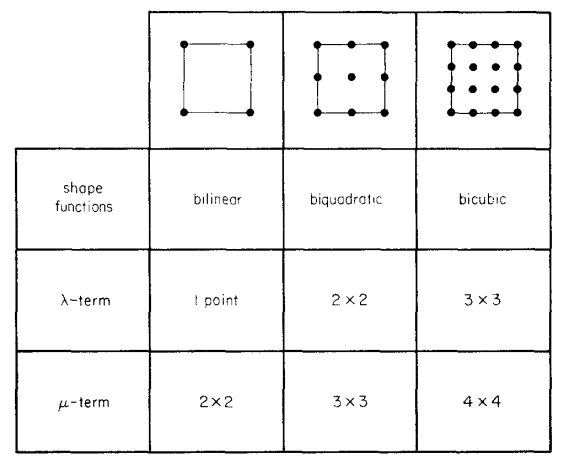
\includegraphics[width=7cm]{images/penalty/hulb79}\\
{\captionfont Selective Gauss-Legendre integration rules for 2-dimensional isoparametric Lagrange
elements. Taken from Hughes \etal (1979) \cite{hulb79}.}
\end{center}

In the context of penalty-based codes, it has been shown \cite{mahu78} that it is crucial to resort 
to a selective reduced integration approach. 
The viscosity term ${\bm A}_{el}^\eta$ is integrated on $2^{ndim}$ points but the 
penalty term ${\bm A}_{el}^\lambda$ must be integrated on a single quadrature point.
Finally, when the pressure is computed from the velocity via Eq.~\eqref{penal}, 
the divergence term must also be computed at a single point in the middle of the element.

See \stone~01 for a concrete example of a 2D penalty-based Stokes solver.

\Literature: Oden \etal \cite{odks82}, Dhatt \& Hubert\cite{dhhu86}.
